\section{Results}
\label{sec:results}

\subsection{Dose--Response on Real Held-Out Data}
\label{sec:dose}

\Figref{fig:dose} and \tabref{tab:main} show the task metric at each ratio.
The three domains follow three different curves.

\begin{figure}[t]
    \centering
    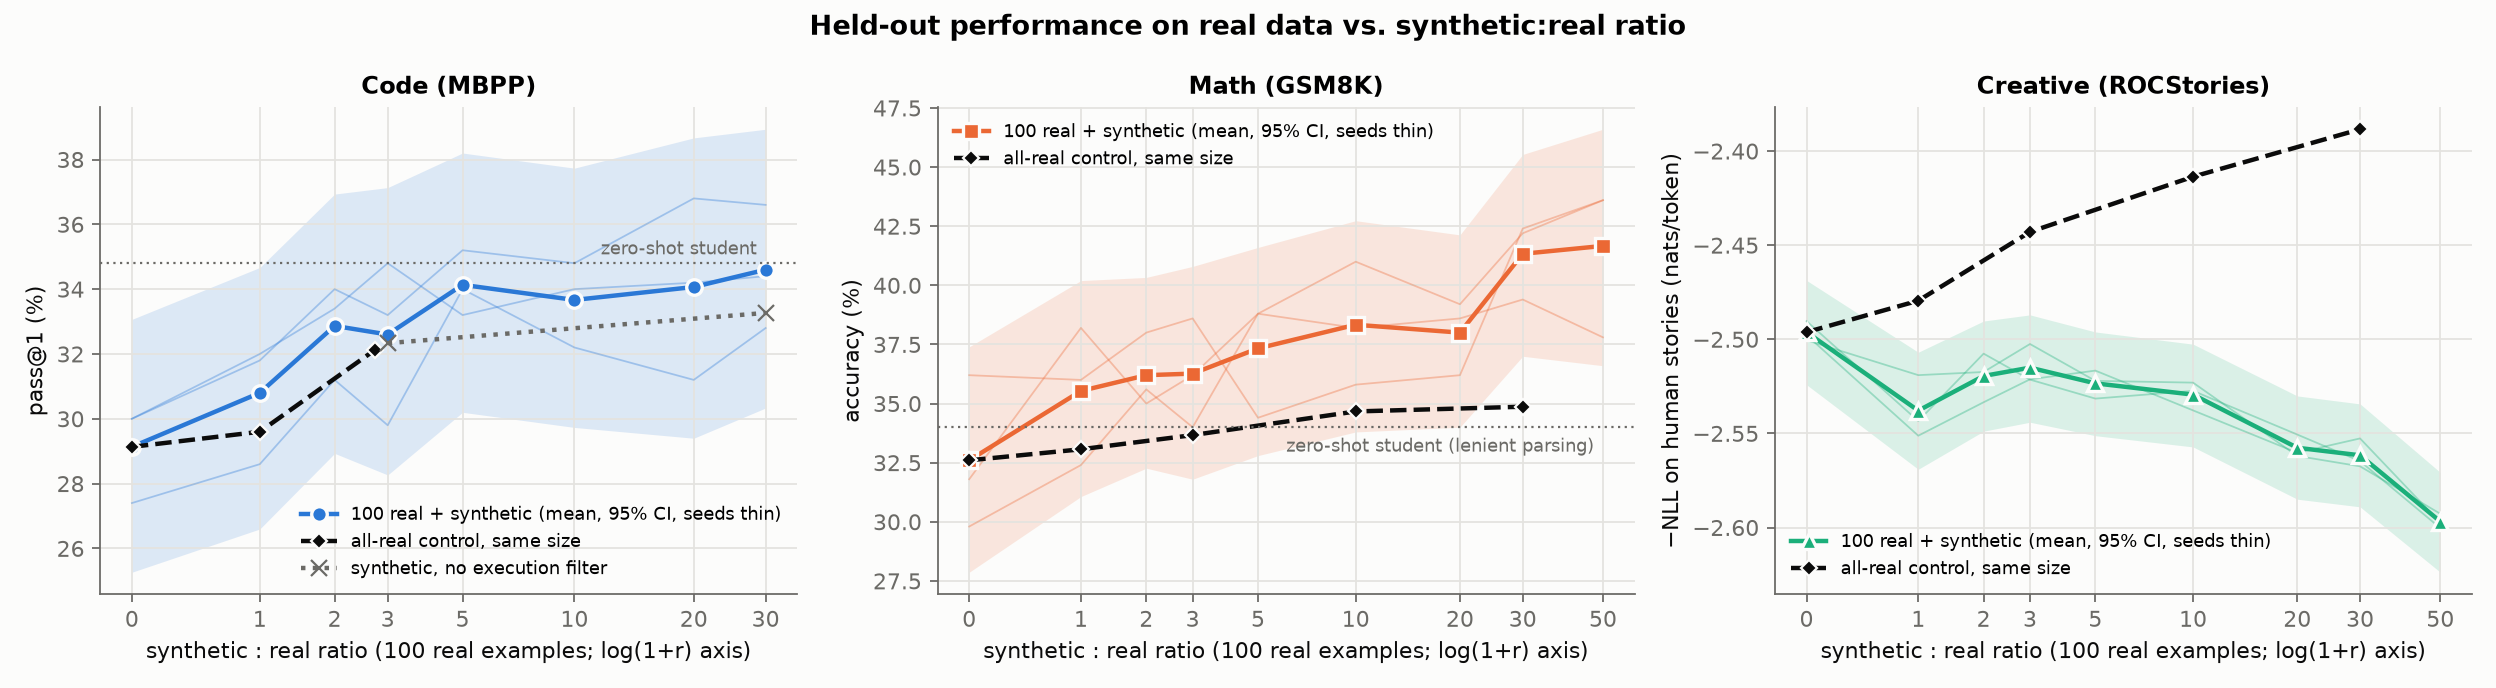
\includegraphics[width=\linewidth]{figures/dose_response.png}
    \caption{Held-out performance on real data against the synthetic-to-real ratio (mean of three seeds; shaded bands are 95\% bootstrap CIs; thin lines are seeds). Black dashed lines show the all-real control at the same training-set size. Code pass@1 rises to about \ratio{5} and then stays flat, never exceeding the zero-shot student. Math accuracy keeps rising to \ratio{50} and exceeds the all-real control. For stories, every synthetic ratio is worse than real-only training, while real data keeps helping.}
    \label{fig:dose}
\end{figure}

\begin{table}[t]
    \centering
    \caption{Task metric on real held-out data (mean of three seeds, 95\% bootstrap CI in brackets). ``Share'' is the normalized benefit $B(r)$ of \eqref{eq:benefit}; it is undefined for creative writing because no ratio beats real-only training. Best value in each ratio sweep in \textbf{bold}. The zero-shot math score uses lenient answer parsing.}
    \label{tab:main}
    \resizebox{\textwidth}{!}{%
    \begin{tabular}{@{}lcccccc@{}}
        \toprule
        & \multicolumn{2}{c}{\codetask (\mbpp)} & \multicolumn{2}{c}{\mathtask (\gsm)} & \creativetask (\roc) \\
        \cmidrule(lr){2-3} \cmidrule(lr){4-5} \cmidrule(lr){6-6}
        \textbf{Ratio} & pass@1 (\%) $\uparrow$ & share & accuracy (\%) $\uparrow$ & share & NLL on human stories $\downarrow$ \\
        \midrule
        0 (real only) & 29.1 \ci{25.3}{33.1} & 0.00 & 32.6 \ci{27.9}{37.4} & 0.00 & \textbf{2.496} \ci{2.469}{2.524} \\
        \ratio{1}  & 30.8 \ci{26.6}{34.7} & 0.30 & 35.5 \ci{31.1}{40.2} & 0.32 & 2.538 \ci{2.507}{2.569} \\
        \ratio{2}  & 32.9 \ci{28.9}{36.9} & 0.68 & 36.2 \ci{32.3}{40.3} & 0.40 & 2.520 \ci{2.490}{2.549} \\
        \ratio{3}  & 32.6 \ci{28.3}{37.1} & 0.63 & 36.3 \ci{31.8}{40.8} & 0.40 & 2.515 \ci{2.487}{2.544} \\
        \ratio{5}  & 34.1 \ci{30.2}{38.2} & 0.91 & 37.3 \ci{32.8}{41.6} & 0.52 & 2.523 \ci{2.496}{2.551} \\
        \ratio{10} & 33.7 \ci{29.7}{37.7} & 0.83 & 38.3 \ci{33.8}{42.7} & 0.63 & 2.529 \ci{2.503}{2.557} \\
        \ratio{20} & 34.1 \ci{29.4}{38.7} & 0.90 & 38.0 \ci{34.0}{42.1} & 0.60 & 2.558 \ci{2.530}{2.585} \\
        \ratio{30} & \textbf{34.6} \ci{30.3}{38.9} & 1.00 & 41.3 \ci{37.0}{45.5} & 0.96 & 2.562 \ci{2.534}{2.589} \\
        \ratio{50} & -- & -- & \textbf{41.7} \ci{36.6}{46.6} & 1.00 & 2.597 \ci{2.571}{2.624} \\
        \midrule
        All-real control, \ratio{3} size & 32.1 (at \ratio{2.74}) & & 33.7 & & 2.443 \\
        All-real control, \ratio{30} size & -- & & 34.9 & & 2.388 \\
        Zero-shot student & 34.8 & & 34.0 & & 2.908 \\
        \bottomrule
    \end{tabular}
    }
\end{table}

\para{Code saturates early.} Pass@1 rises from 29.1\% with real data only to 34.1\% at \ratio{5} and then moves by less than a point up to \ratio{30} (34.6\%).
Real-only fine-tuning makes the student \emph{worse} than zero-shot (29.1\% against 34.8\%), and the best synthetic condition only recovers to parity.
On \mbpp the benefit we measure is therefore recovery from a harmful real-only baseline, not an improvement over the untuned model.

\para{Math keeps improving.} Accuracy rises from 32.6\% to 36.3\% at \ratio{3}, 38.3\% at \ratio{10}, and 41.7\% at \ratio{50}.
The all-real control improves far less, from 32.6\% to 34.9\% at the \ratio{30} size.

\para{Stories get worse from the first synthetic example.} The NLL on human stories is lowest with no synthetic data (2.496) and rises to 2.597 at \ratio{50}.
The all-real control moves the other way, to 2.388 at the \ratio{30} size.

\subsection{Does a \ratio{3} Ratio Capture 80\% of the Benefit?}
\label{sec:h1b}

No.
The share of maximum observed gain at \ratio{3} is 0.63 for code (95\% CI 0.13--1.00) and 0.40 for math (CI 0.06--0.64).
The math interval excludes 0.8, and the share reaches 0.8 in only 0.2\% of bootstrap resamples for math and 14\% for code.
Code first reaches 80\% of its maximum at about \ratio{5}.
For math the maximum sits at the edge of the grid, so 0.40 is an upper bound on the true share.
For creative writing the share is undefined because no ratio beats real-only training.
The left panel of \figref{fig:normalised} shows the full curves.

\begin{figure}[t]
    \centering
    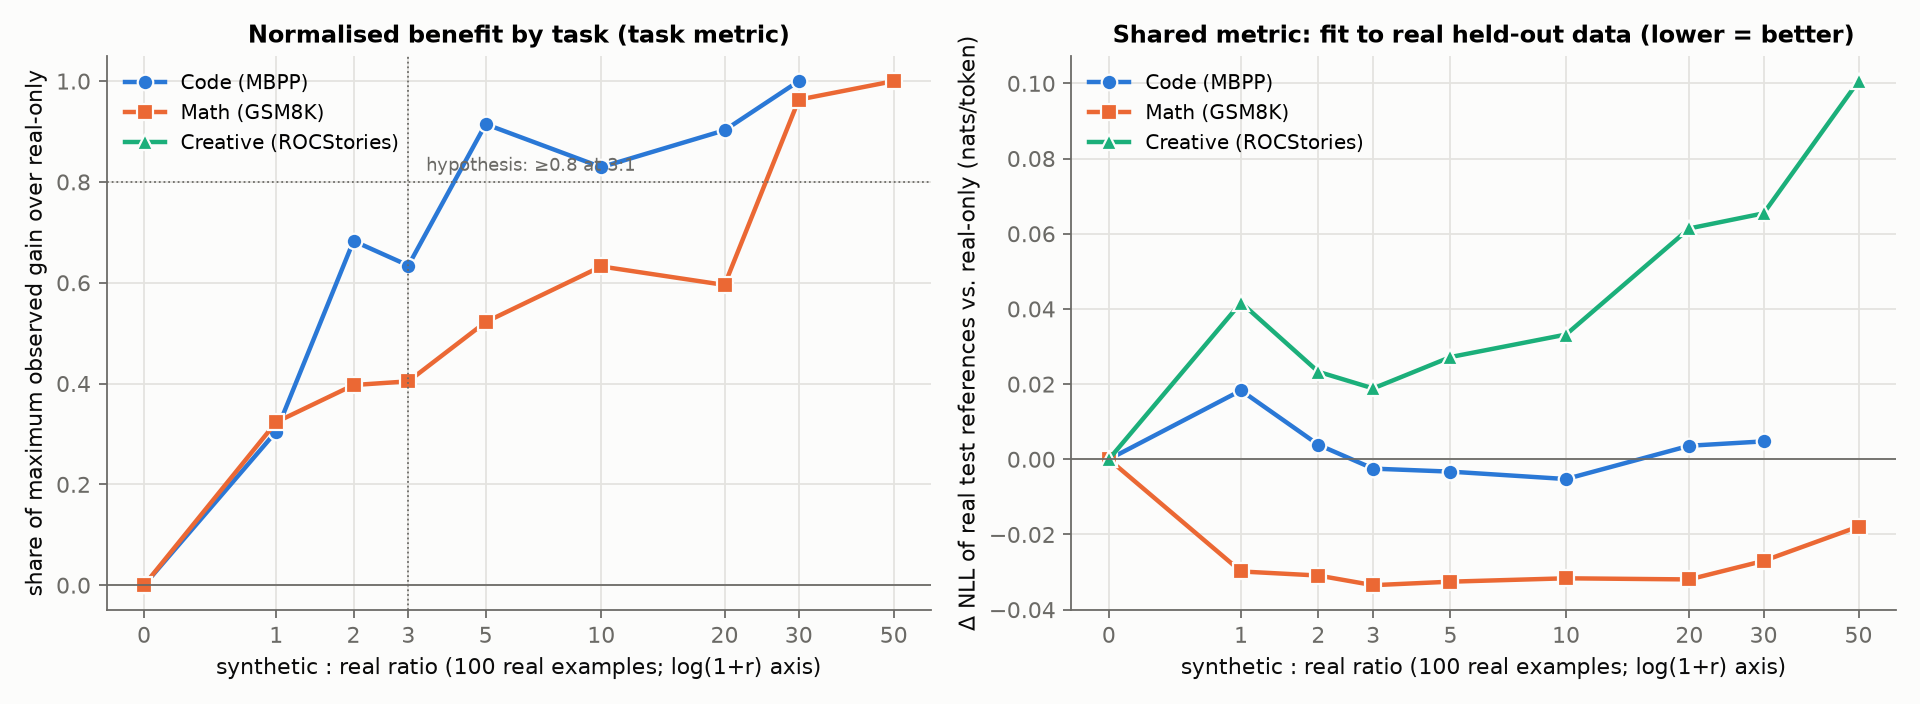
\includegraphics[width=0.95\linewidth]{figures/normalised_benefit.png}
    \caption{\figleft Share of the maximum observed gain on the task metric. The hypothesis predicts at least 0.8 at \ratio{3} (dotted lines); code reaches 0.63 and math 0.40. \figright Change in NLL on real held-out references relative to real-only training (lower is better). All three tasks degrade beyond \ratio{10}; the degradation for stories is an order of magnitude larger than for code and math.}
    \label{fig:normalised}
\end{figure}

\subsection{What Happens Beyond \ratio{10}?}
\label{sec:h2a}

\begin{table}[t]
    \centering
    \caption{Planned contrasts on the task metric: difference with 95\% CI. Code and math are in accuracy points. Creative writing is in $-$NLL (nats per token), so negative values mean a worse fit to human stories. $^{*}$ $p < 0.05$, $^{***}$ $p < 0.001$ (Holm-adjusted across tasks; unadjusted for the \ratio{50} contrast); unmarked contrasts are not significant.}
    \label{tab:contrasts}
    \begin{tabular}{@{}llll@{}}
        \toprule
        \textbf{Contrast} & \codetask (points) & \mathtask (points) & \creativetask ($-$NLL) \\
        \midrule
        \ratio{3} $-$ real-only & $+3.5^{*}$ \ci{+0.7}{+6.5} & $+3.7^{*}$ \ci{+0.6}{+6.8} & $-0.019^{*}$ \ci{-0.031}{-0.004} \\
        \ratio{10} $-$ \ratio{3} & $+1.1$ \ci{-1.9}{+3.8} & $+2.1$ \ci{-3.0}{+6.7} & $-0.014^{***}$ \ci{-0.021}{-0.007} \\
        \ratio{30} $-$ \ratio{10} & $+0.9$ \ci{-1.6}{+3.6} & $+3.0$ \ci{-1.0}{+7.3} & $-0.032^{***}$ \ci{-0.044}{-0.016} \\
        \ratio{50} $-$ \ratio{10} & -- & $+3.3$ \ci{-1.6}{+8.4} & $-0.067^{***}$ \ci{-0.074}{-0.060} \\
        \bottomrule
    \end{tabular}
\end{table}

\para{On the task metric, the answer depends on the domain.}
\Tabref{tab:contrasts} gives the planned contrasts.
For code, \ratio{30} differs from \ratio{10} by $+0.9$ points (CI $-1.6$ to $+3.6$), and the slope of pass@1 per unit of $\ln r$ for $r \geq 10$ is $+0.8$ points (CI $-1.5$ to $+3.3$): a plateau.
For math, accuracy at \ratio{30} and \ratio{50} is 3.0 and 3.3 points above \ratio{10}, and the slope is $+2.4$ points per unit of $\ln r$ (CI $-0.8$ to $+5.8$).
Neither math contrast is individually significant, so we detect no plateau but cannot exclude one.
For stories, every step is a significant loss, with a slope of $-0.040$ nats per unit of $\ln r$ (CI $-0.044$ to $-0.033$).

\para{On the shared metric, all three domains degrade.}
\Tabref{tab:nll} and the right panel of \figref{fig:normalised} show the NLL on real held-out references.
All three tasks have an interior optimum followed by degradation: the best ratio is \ratio{10} for code, \ratio{3} for math, and 0 for stories.
From \ratio{10} to \ratio{30} the NLL rises by 0.0100 nats for code, 0.0046 for math, and 0.0322 for stories, each with $p < 0.001$.
The degradation is small for code and math (at most 0.01 nats) and an order of magnitude larger for stories.
Math shows both effects at once: accuracy rises with the ratio while the fit to human-written reference solutions is best at \ratio{3} and then worsens.

\begin{table}[t]
    \centering
    \caption{Shared metric: NLL of real held-out references (nats per token; positive differences mean a worse fit). ``Best ratio'' gives the ratio with the lowest mean NLL and the share of bootstrap resamples in which it is best.}
    \label{tab:nll}
    \resizebox{0.9\textwidth}{!}{%
    \begin{tabular}{@{}llcc@{}}
        \toprule
        \textbf{Task} & \textbf{Best ratio} & \textbf{\ratio{30} $-$ \ratio{10}} & \textbf{\ratio{30} $-$ real-only} \\
        \midrule
        \codetask & \ratio{10} (85\%) & $+0.0100$ \ci{+0.0037}{+0.0183}, $p < 0.001$ & $+0.0048$ \ci{-0.0018}{+0.0119}, \ns \\
        \mathtask & \ratio{3} (61\%) & $+0.0046$ \ci{+0.0025}{+0.0069}, $p < 0.001$ & $-0.0270$ \ci{-0.0521}{-0.0067}, $p < 0.001$ \\
        \creativetask & 0 (99\%) & $+0.0322$ \ci{+0.0158}{+0.0442}, $p < 0.001$ & $+0.0654$ \ci{+0.0551}{+0.0756}, $p < 0.001$ \\
        \bottomrule
    \end{tabular}
    }
\end{table}

\subsection{Are Gains Logarithmic?}
\label{sec:h1a}

Only for math, and weakly.
\Tabref{tab:fits} compares the five curve families.
For math the logarithmic model has the lowest AICc, but it explains little variance ($R^2 = 0.28$) and the power law is within 1.6 units.
For code, bounded saturating curves fit best and the logarithmic model is 11.4 AICc units worse.
For stories the ``gain'' is negative, and a power law describes the loss best.
A linear model is the worst fit in all three domains.

\begin{table}[t]
    \centering
    \caption{Curve fits to seed-level gains: $\Delta$AICc (0 = best, in \textbf{bold}) with $R^2$ in parentheses. No single functional form wins across domains.}
    \label{tab:fits}
    \begin{tabular}{@{}lccccc@{}}
        \toprule
        \textbf{Task} & \textbf{Linear} & \textbf{Log} & \textbf{Power} & \textbf{Hyperbolic} & \textbf{Exp.\ saturation} \\
        \midrule
        \codetask & 37.7 ($-2.03$) & 11.4 (0.13) & 4.5 (0.45) & 0.6 (0.55) & \textbf{0.0} (0.56) \\
        \mathtask & 12.3 ($-0.21$) & \textbf{0.0} (0.28) & 1.6 (0.31) & 2.9 (0.27) & 4.1 (0.23) \\
        \creativetask & 14.3 (0.41) & 4.4 (0.61) & \textbf{0.0} (0.71) & 8.0 (0.60) & 9.4 (0.57) \\
        \bottomrule
    \end{tabular}
\end{table}

\subsection{Mechanism: Diversity of the Synthetic Pools}
\label{sec:diversity}

\begin{figure}[t]
    \centering
    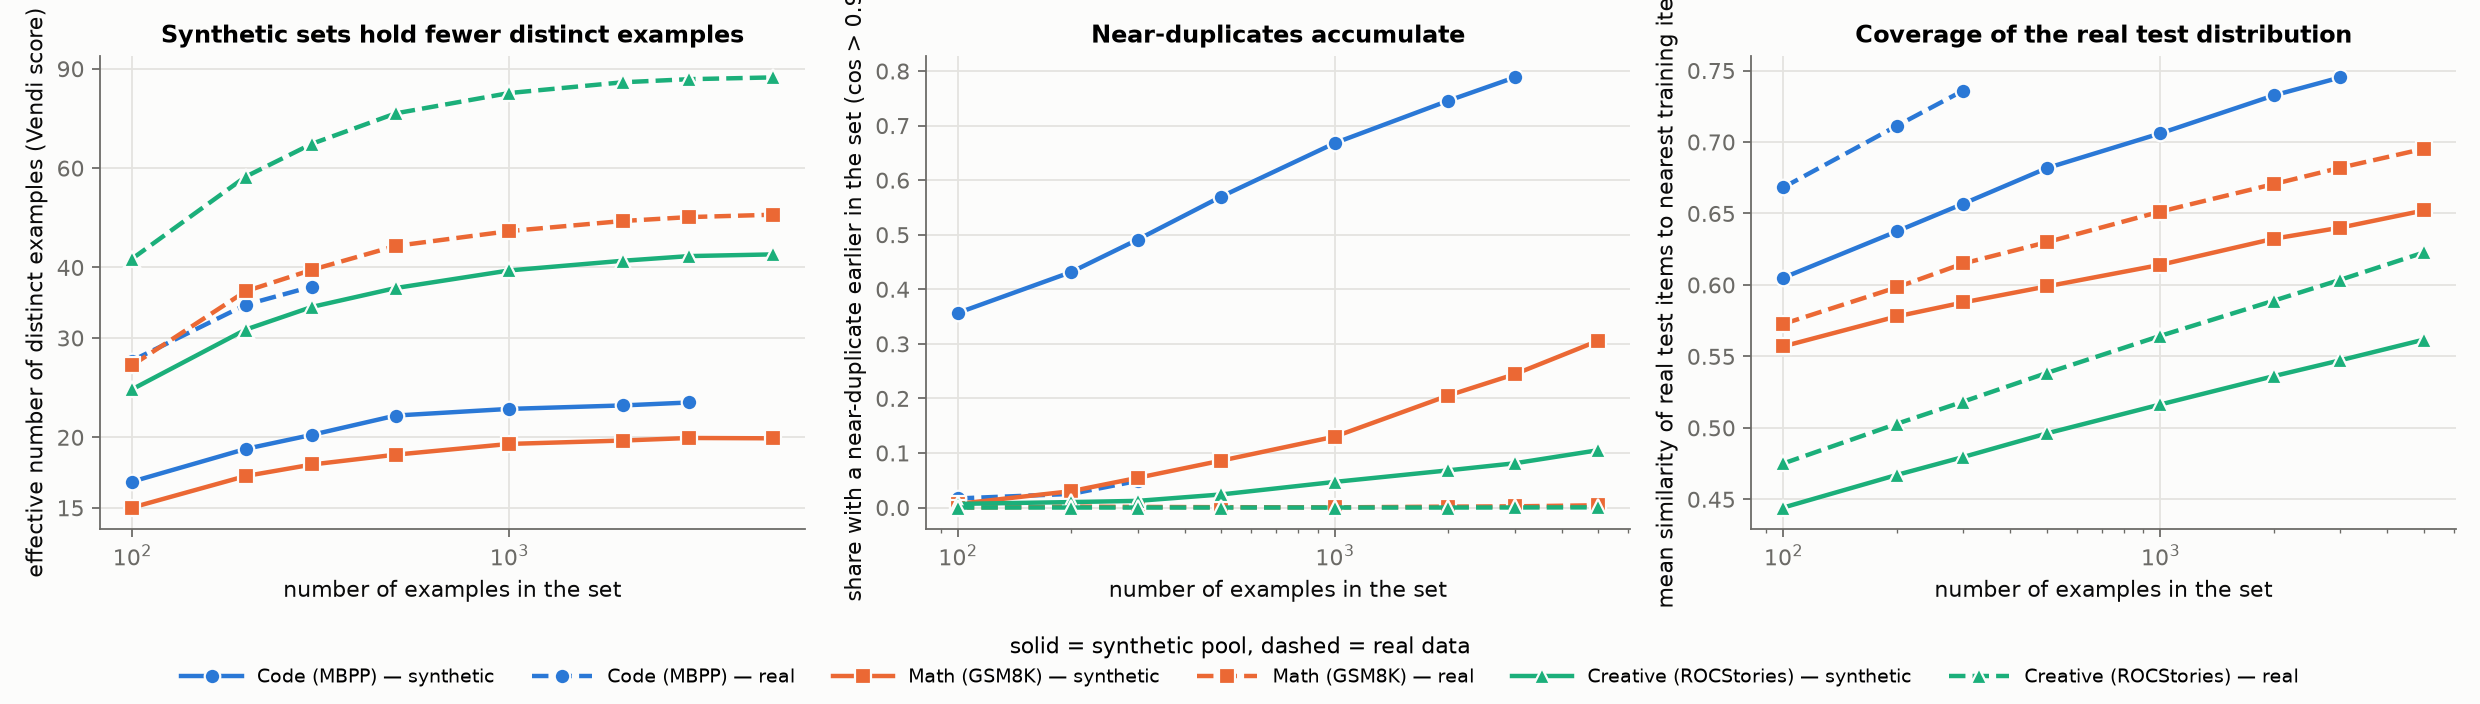
\includegraphics[width=\linewidth]{figures/pool_diversity.png}
    \caption{Diversity of synthetic pools (solid) and real data (dashed) as the set grows. \figleft The effective number of distinct examples (Vendi score) saturates for synthetic pools well below the level of real data. \figcenter Near-duplicates accumulate in synthetic pools, fastest for code, and are nearly absent in real data. \figright Synthetic data covers the real test distribution less well than real data at every size.}
    \label{fig:diversity}
\end{figure}

\begin{table}[t]
    \centering
    \caption{Diversity of synthetic pools and real data (mean over three pools). Near-duplicates have cosine similarity above 0.9 to an earlier example. ``Vendi'' is an effective number of distinct examples in embedding space. ``Coverage'' is the mean similarity of real test items to their nearest training example.}
    \label{tab:diversity}
    \resizebox{\textwidth}{!}{%
    \begin{tabular}{@{}llrccccc@{}}
        \toprule
        \textbf{Task} & \textbf{Source} & $n$ & \textbf{Exact dup.} & \textbf{Near-dup.} & \textbf{Distinct bigrams} & \textbf{Vendi} & \textbf{Coverage} \\
        \midrule
        \multirow{3}{*}{\codetask} & synthetic & 300 & 22\% & 49\% & 0.21 & 20.2 & 0.657 \\
         & synthetic & 3,000 & 44\% & 79\% & 0.08 & 23.1 & 0.745 \\
         & real & 300 & 0\% & 5\% & 0.37 & 37.0 & 0.736 \\
        \midrule
        \multirow{3}{*}{\mathtask} & synthetic & 300 & 0\% & 5\% & 0.43 & 17.9 & 0.588 \\
         & synthetic & 5,000 & 0.2\% & 31\% & 0.15 & 19.9 & 0.652 \\
         & real & 5,000 & 0\% & 0.4\% & 0.39 & 49.6 & 0.695 \\
        \midrule
        \multirow{3}{*}{\creativetask} & synthetic & 300 & 0\% & 1\% & 0.62 & 34.1 & 0.480 \\
         & synthetic & 5,000 & 0\% & 11\% & 0.30 & 42.2 & 0.562 \\
         & real & 5,000 & 0\% & 0.0\% & 0.42 & 86.9 & 0.623 \\
        \bottomrule
    \end{tabular}
    }
\end{table}

{\bf Does the generator collapse onto a few modes?} Yes.
\Tabref{tab:diversity} and \figref{fig:diversity} compare synthetic pools with real data.
In a 3,000-example code pool, 44\% of task descriptions are exact duplicates and 79\% have a near-duplicate, against 0\% and 5\% for 300 real \mbpp problems.
In the seed-0 pools, \texttt{factorial} is the function in 523 of 3,626 usable code examples (14\%) and \texttt{fibonacci} in 197; 1,232 of 5,174 math problems (24\%) begin with ``Sarah''; and story titles concentrate on variants of ``The Book Swap'' (257), ``The Lost Key'' (256), and ``Birthday Surprise'' (159).

Growing a pool adds little that is new.
Going from 300 to 3,000--5,000 synthetic examples raises the Vendi score by only 14\% for code, 11\% for math, and 24\% for stories.
At 5,000 examples the Vendi score of synthetic data is 40\% of that of real data for math (19.9 against 49.6) and 49\% for stories (42.2 against 86.9).
Synthetic data needs roughly 5--10 times as many examples as real data to reach the same coverage of the real test set: 5,000 synthetic math problems reach the coverage of 1,000 real ones (0.652 against 0.651), and 3,000 synthetic code tasks reach that of 300 real ones (0.745 against 0.736).

The code pools are the most collapsed, and code is the domain where accuracy saturates earliest.
This is consistent with H2b: beyond about \ratio{5} a larger code pool adds almost no new problems.
The evidence is correlational, because we do not vary diversity at fixed pool size.

\subsection{What the Student Writes}
\label{sec:creative}

\begin{figure}[t]
    \centering
    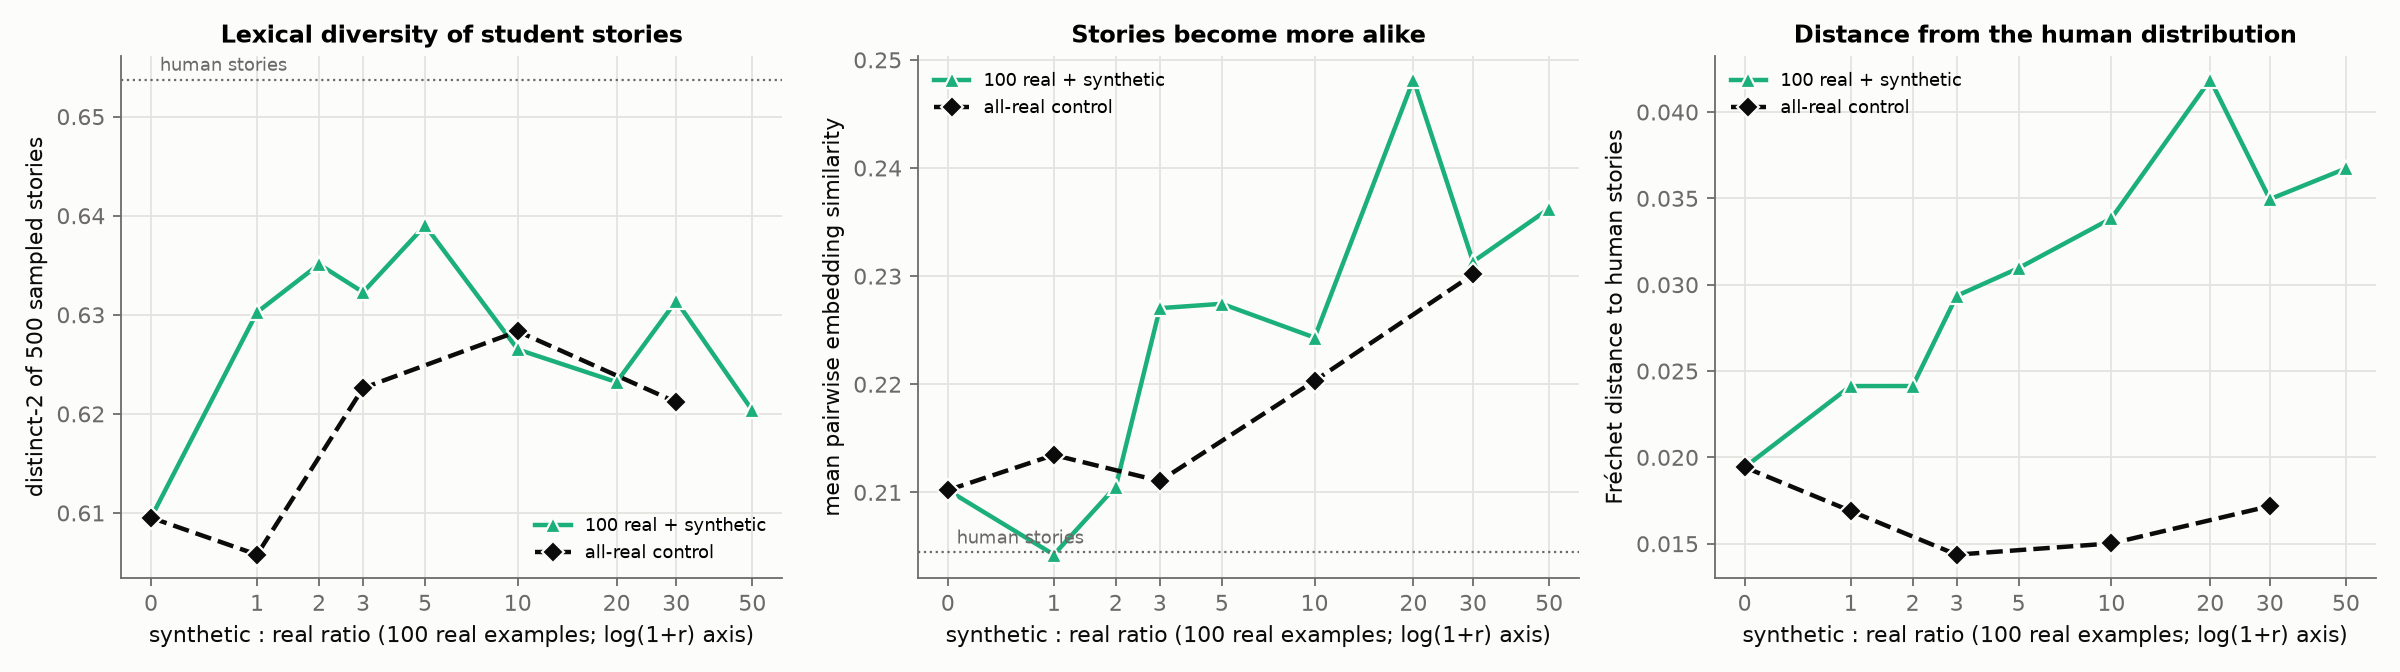
\includegraphics[width=\linewidth]{figures/creative_generation.png}
    \caption{Properties of 500 sampled student stories per model. \figleft Lexical diversity (distinct-2) does not fall with the synthetic ratio. \figcenter Stories become more similar to each other in embedding space. \figright The Fr\'echet distance to human stories roughly doubles with synthetic data, while the all-real control stays near the noise floor of 0.013.}
    \label{fig:creative}
\end{figure}

\begin{table}[t]
    \centering
    \caption{Properties of 500 sampled student stories (mean over seeds). The Fr\'echet distance reported for human stories is the noise floor of the estimate. Values closest to human stories among trained students in \textbf{bold}.}
    \label{tab:creative}
    \resizebox{0.95\textwidth}{!}{%
    \begin{tabular}{@{}lcccc@{}}
        \toprule
        \textbf{Condition} & \textbf{Distinct-2} & \textbf{Pairwise similarity} & \textbf{Fr\'echet distance} $\downarrow$ & \textbf{Five sentences} \\
        \midrule
        Human stories & 0.654 & 0.204 & 0.013 & 99.8\% \\
        \midrule
        Real only ($r = 0$) & 0.610 & \textbf{0.210} & 0.019 & 69\% \\
        Synthetic \ratio{3} & \textbf{0.632} & 0.227 & 0.029 & 77\% \\
        Synthetic \ratio{30} & 0.631 & 0.231 & 0.035 & 70\% \\
        Synthetic \ratio{50} & 0.620 & 0.236 & 0.037 & 77\% \\
        All-real control, \ratio{30} size & 0.621 & 0.230 & \textbf{0.017} & \textbf{98\%} \\
        \bottomrule
    \end{tabular}
    }
\end{table}

\Tabref{tab:creative} and \figref{fig:creative} describe the stories that students sample.
The Fr\'echet distance to human stories rises from 0.019 with real data only to 0.035 at \ratio{30} and 0.037 at \ratio{50}; the all-real control at the \ratio{30} size stays at 0.017.
Only the all-real control learns the format: 98\% of its stories have exactly five sentences, against 69--77\% for the other conditions.

\para{Lexical diversity does not collapse.} Distinct-2 of student stories is not lower with synthetic data (0.62--0.64 against 0.61 for real-only).
The homogenization shows up in content: mean pairwise embedding similarity rises from 0.210 to 0.236 at \ratio{50}, and stories converge on the teacher's preferred names and scenarios.
The all-real control at the \ratio{30} size also reaches a pairwise similarity of 0.230, so this statistic alone does not separate synthetic from real training; the Fr\'echet distance and the inherited modes below do.

\para{Students inherit the teacher's modes.} We count occurrences of the name ``Sarah'' in 500 stories (seed 0).
Human test stories contain 8 and the first 500 synthetic stories contain 375.
The student contains 11 after real-only training, 13 after the all-real control, and 171 after \ratio{30} training, a 15-fold increase.
For the title ``Kitchen Table'', the all-real student writes: \emph{``Jane was creating a remodel for her home. She wanted to make the kitchen. She did a great job with the room. She showed her neighbors. They said the kitchen looked pretty.''}
The \ratio{30} student writes: \emph{``At the kitchen table, Sarah decided to bake a cake. She placed all her ingredients on a rimmed baking sheet. Unexpectedly, the hot baking sheets melted away. Relieved, she let the cake cool, then took a photo to show her husband.''}

\subsection{Synthetic Against Real Data at Equal Size}
\label{sec:synth_vs_real}

The all-real control separates the source of the data from its amount (\tabref{tab:synth_real} in the appendix).
For stories, real data wins at every size, and the gap grows from 0.058 nats at the \ratio{1} size to 0.173 at the \ratio{30} size.
For math, the synthetic mix wins on accuracy, and the gap also grows: $+3.7$ points at the \ratio{10} size (CI $+0.4$ to $+7.0$, $p = 0.030$) and $+6.5$ points at the \ratio{30} size (CI $+2.3$ to $+11.0$, $p = 0.002$).
This holds even though the all-real model fits the real references far better (NLL 0.637 against 0.682).
For code the control only extends to \ratio{2.74}, where real data scores 32.1\% against 32.6\% for the synthetic mix at \ratio{3}.

\subsection{Error Analysis and Ablation}
\label{sec:errors}

\para{Code.} Wrong answers dominate failures: 52--55\% of test items raise an assertion error at every ratio. From real-only to \ratio{30}, synthetic data reduces other runtime errors from 4.6\% to 2.5\% of items and wrong answers from 55.0\% to 51.9\%, while syntax errors stay near 1\%. The zero-shot student makes more syntax errors (5.0\%) but fewer wrong answers (48.0\%).

\para{Math.} Almost all failures are wrong final answers, which fall from 66\% of items with real data only to 55\% at \ratio{50}. Format failures (no answer line) stay between 1\% and 6\%.

\para{Execution filter.} Without the execution filter on the code pool, pass@1 is 32.3\% at \ratio{3} and 33.3\% at \ratio{30}, against 32.6\% and 34.6\% with it. The per-seed differences at \ratio{30} go both ways ($+0.2$, $-1.4$, $+5.2$ points), so the ablation is inconclusive.
